%\documentclass[13pt]{article}
\documentclass{article}
\usepackage[utf8]{inputenc}

\usepackage{amssymb}
\usepackage{amsthm}
\usepackage{amsxtra}
\usepackage{amsmath}
\usepackage{amscd}
\usepackage{epstopdf}
\usepackage[ruled,vlined]{algorithm2e}
%\usepackage[T1]{fontenc}
%\usepackage[french]{babel}
\usepackage{cite}
\usepackage{url}
\usepackage[hidelinks]{hyperref}
\usepackage{tikz}

\theoremstyle{plain} % style plain
\newtheorem{theorem}{Theorem}[section]
\newtheorem{lemma}[theorem]{Lemma}
\newtheorem{conjecture}[theorem]{Conjecture}
\newtheorem{proposition}[theorem]{Proposition}
\newtheorem{property}[theorem]{Proposition}
\newtheorem{corollary}[theorem]{Corollary}
\newtheorem{fact}[theorem]{Fact}
\newtheorem{claim}[theorem]{Claim}
\newtheorem{problem}[theorem]{Problem}
\theoremstyle{definition} % style definition

\newtheorem{definition}[theorem]{Definition}
\newtheorem{assumption}[theorem]{Assumption}
\newtheorem{invariant}[theorem]{Invariant}
\newtheorem{example}{Example}[section]
\newtheorem*{notation}{Notation}
\newtheorem*{convention}{Convention}
\newtheorem*{note}{Note}
\newtheorem{remark}[theorem]{Remark}
\newtheorem{observation}[theorem]{Observation}


\title{Steiner tree problem}
\date{\today}
\author{Antoine Huchet}

\begin{document} \maketitle

\tableofcontents
\newpage

\section{Problem description}

We are going to study the Steiner tree problem, which is defined as
follows: Given a graph $G=(V,E)$, a weight function $w: e \mapsto \mathbb{R}$
assigning a weight w(e) for every $e \in V$  and a set of terminal nodes $T
\subset V$. The goal is to find a subset of edges $M \subset E$ of minimal
weight that connects all terminals in $G$.

This problem is \textsc{np-complete}. Here we are going to be presenting and
comparing different heuristic approaches to the problem.

\section{Definition}

\subsection{Checking admissibility}

\begin{definition}
Since a solution needs to connect all terminal nodes, I will define a solution
to be admissible when all terminal nodes $t \in T$ are in the same connected
component.
\end{definition}

\subsection{Gain function}

\begin{definition}
My gain function will simply be the sum of all edges plus the diameter of the
graph.
\end{definition}

The diameter being the maximum eccentricity over all vertices. The
eccentricity of a vertex being the distance (shortest path over the weighted
edges) from that vertex to the furthest away vertex.

\begin{remark}
Note that the leaves of an optimal solution will necessarily be terminals.
\end{remark}

\section{Overview}

The basic framework I will use is the one seen in class.

\begin{itemize}
\item First, I will initialise a solution from a known approximation algorithm.

\item Then I will generate new solutions by considering variations of my
current solutions.

\item Finally I will select a few solutions from which I will iterate,
optimizing the gain function.

\item I will stop after a fixed amount of iterations.
\end{itemize}

\begin{algorithm}

\caption{\textsc{generic\_framework} ($\lambda$, $\mu$, \textsc{variation},
\textsc{selection}, $k$, $G$, $T$)}

Sample $\mu$ first feasible solutions $x_1,\ldots,x_\mu$ based on a known
approximation algorithm.\\

\While{number\_iterations $< k$}{\
	$\{x_1,\ldots,x_\lambda\} =$ \textsc{variation}(T,
					$\{x_1,\ldots,x_\mu\}$, $\lambda$) \\

	$\{x_1,\ldots,x_\mu\} = $ \textsc{selection}($\{x_1,\ldots,x_{\lambda +
							\mu}\}$, $\mu$)\\
	%Create $\lambda$ variations $x_1,\ldots,x_\lambda$ based on the $\mu$
	%previous solutions.\\
	%Select $\mu$ solutions.\\
}
\Return $x$ that minimizes the gain function.

\end{algorithm}

\begin{itemize}

\item $\lambda$ being the number of variations I am considering.

\item $\mu$ being the number of solutions I am selecting.

\item $\textsc{variation}$ being a function used to consider variations of the
current solutions.

\item $\textsc{selection}$ being a function used to select $\mu$ solutions from
the current solutions.

\item $k$ is a simple integer, $G$ our graph and $T$ our terminal nodes.

\end{itemize}


\section{Initialisation}

The problem will be initialised by the following 2-apprximation algorithm.

For all pair of terminals, compute the shortest path between all pair of
terminal vertices. Then return the minimum spanning tree of this subgraph.

This algorithm is clearly correct as terminal nodes are never disconnected from
the connected component.

\begin{remark} I will admit that it is a 2-approximation as I don't want my
report to be 20 pages and all that really matters is that it yields an
admissible solution.
\end{remark}

\section{Variation}

Here I will present the different ways of generating a new solution based on
already computed solutions that I studied.

\subsection{Mutation}

I will refer as mutation all variations that modify a solution by only changing
it a little bit.

\subsubsection{Adding an edge}

A straight-forward mutation that could be applied to an admissible solution
would be adding an edge. The edge should have one end in the current solution
as we have no interest in creating another connected component. The solution
will obviously stay admissible as no terminal nodes can be disconnected from
that operation.

This operation sounds quite limited as it doesn't change the solution much.
Therefore, we might want to modify the solution more to bypass those potential
local optimums.

\subsubsection{Adding a path}

Another mutation that would be worth considering is adding a whole path to
our current solution. In order to do so, we would randomly select two nodes
from out curent solution then add a shortest path based on the graph $G$ we
started with.

This mutation is interesting as it changes the solution significantly.
Solutions look better than the previous solution.

\subsubsection{Clean the solution}

After either of the previous two mutations, it is interesting to remove as many
unnecessary edges as possible. An unnecessary edge is an edge that when removed
doesn't make the solution unfeasible.

Unnecessary edges are removed in a random order.

This operation is more time consuming as it would entail checking if the
solution is still feasible for each edge.

\subsubsection{Multiple mutation}

\begin{definition}[Multiple mutation]
With a probability $p$ add an edge, with probability $1-p$ add a path then
clean the solution.
\end{definition}

\subsection{Crossover}

I will refer as crossover a variation that merges from two previous solutions.

The crossover mutation I will consider is merging two solutions $S_1 = (V_1,
E_1)$ and $S_2 = (V_2, E_2)$ into $S = (V_1 \cup V_2,E_1 \cup E_2)$ then
cleaning it as explained above.

\subsection{Combining both}

Another variation that I will consider is a mix of both a mutation and a
crossover. Depending on how many offsprings we request, I will generate a
multiple mutation then a crossover then a crossover on a multiple mutation.

This yields good variations of our current set of solutions.

\section{Selection}

In this section I will be presenting different ways of selecting solutions.

\subsection{Elitist selection}

The elitist selection will sample the best $\mu$ solutions out of the $\lambda
+ \mu$ solutions.

\subsection{Elitist selection on offsprings only}

The elitist selection on offsprings only will sample the $\mu$ best solutions
out of the $\lambda$ offpsrings.

It could be a problem when $\lambda < \mu$. If this happens, it will fall back
to the previous elitist selection.

\subsection{Fitness proportional selection}

The fitness proportional selection samples $\mu$ solutions with probability
proportional to their gain such that the solution that is the closest to the
optimum has the highest probability of being chosen.

From my experience, this doesn't work very well as our solutions tend to have a
relatively high gain (a few thousands) and aren't very far from each other (a
few hundreds). Therefore the probability vector that I compute is close to
uniform.

A workaround could be to compute the probability vector based only on the
distance to the current best solution so that the probabilities aren't so close
to uniform.

\subsection{Boltzmann selection}

The Boltzmann selection samples $\mu$ solutions out of the $\lambda$
offsprings. It selects an offspring $x$ if it is better than the best previous
solutions $y$. If it is worse, it selects it with probability $e^{\frac{gain(x)
- gain(y)}{T}}$. For some value of T.

\subsection{Threshold selection}

The Threshold selection samples $\mu$ solutions out of the $\lambda$
offsprings. It selects an offspring $x$ if it is better than the best previous
solutions $y$. If it is worse, it selects it with probability $gain(x) >
gain(y) + T$. For some value of $T$.

In my experiments, $T$ is constant. It would be a good idea to have it follow a decreasing sequence of the form $e^{-x}$.

\section{Comparison}

Here I will be comparing the variation and selection strategies.

\subsection{Variations}

In figure~\ref{Mutationcompareselection}, as predicted, the fitness
proportional is too uniform therefore doesn't get neither better nor worse.  It
looks like the threshold variation isn't converging very quickly either.  Maybe
my $T$ parameter was a little too big.
\\
In figure~\ref{Crossovercompareselection}, except for the fitness proportional
selection, it looks like we are converging rather quickly to a not so great
solution.
\\
In figure~\ref{Multiplecompareselection}, we observe that combining both
variations yields interesting results.

%MUTATION
\begin{figure}
\centering
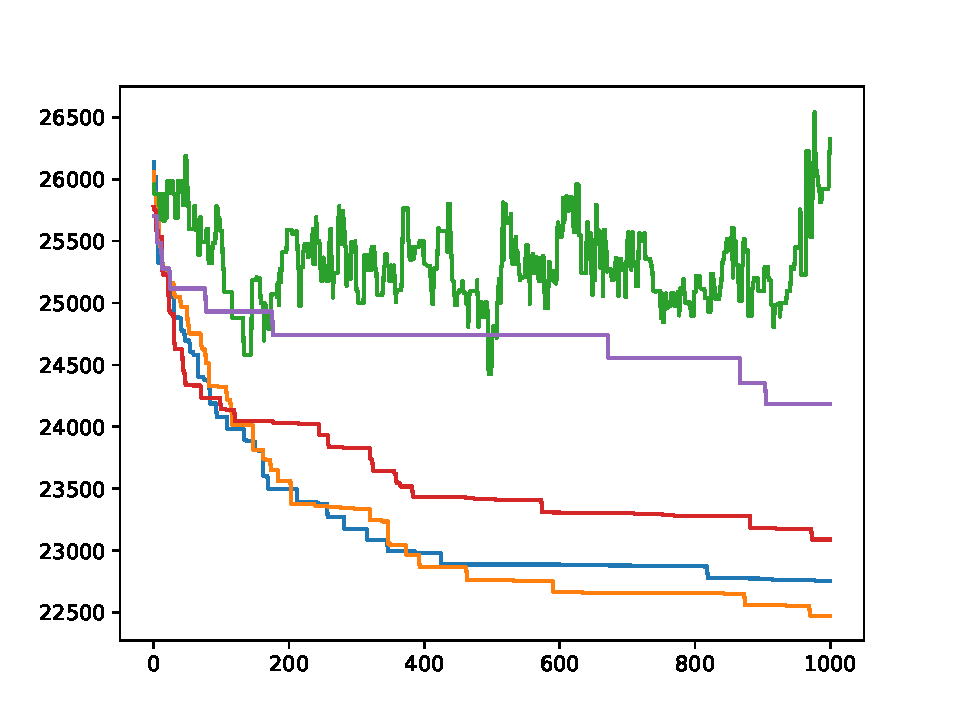
\includegraphics[scale=.6]{../Plots/new/5,2,mutation,eofb1000t-150.pdf}
\caption{Comparaison for $\lambda = 5$, $\mu = 2$ and mutation variation of
classic elitist selection (in blue), elitist selection on offsprings (in
orange), fitness proportional (in green), Boltzmann with constant $T = 1000$
(in red) and Threshold selection with constant parameter $T = -150$ (in
purple)}
\label{Mutationcompareselection}
\end{figure}

%CROSSOVER
\begin{figure}
\centering
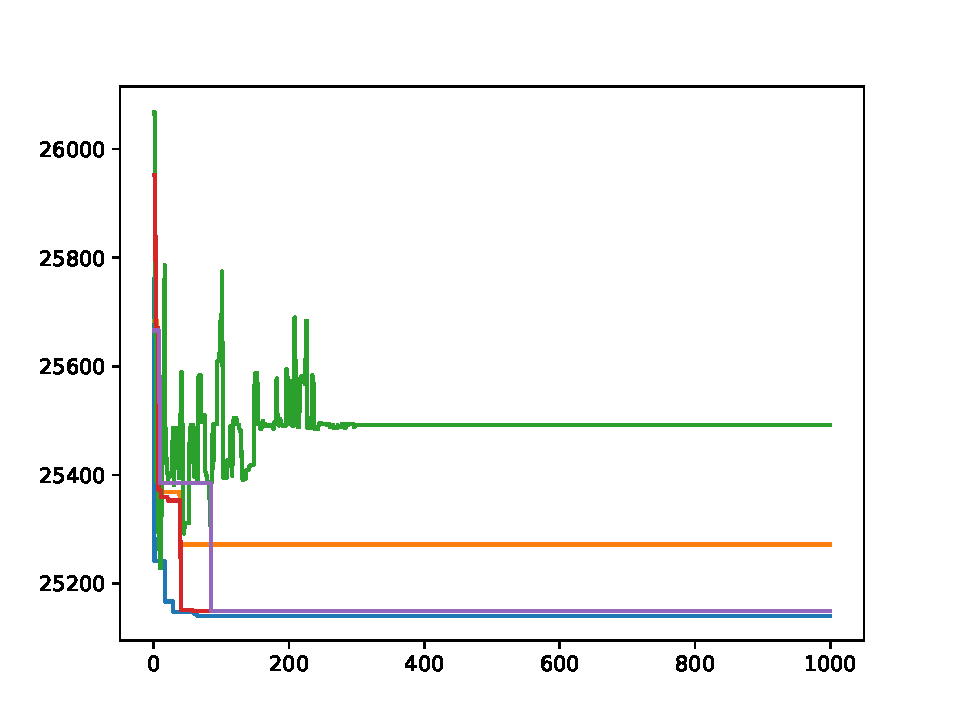
\includegraphics[scale=.6]{../Plots/new/5,2,crossover,eofb1000t-150.pdf}
\caption{Comparaison for $\lambda = 5$, $\mu = 2$ and crossover variation of
classic elitist selection (in blue), elitist selection on offsprings (in
orange), fitness proportional (in green), Boltzmann with constant $T = 1000$
(in red) and Threshold selection with constant parameter $T = -150$ (in
purple)}
\label{Crossovercompareselection}
\end{figure}

%MULTIPLE
\begin{figure}
\centering
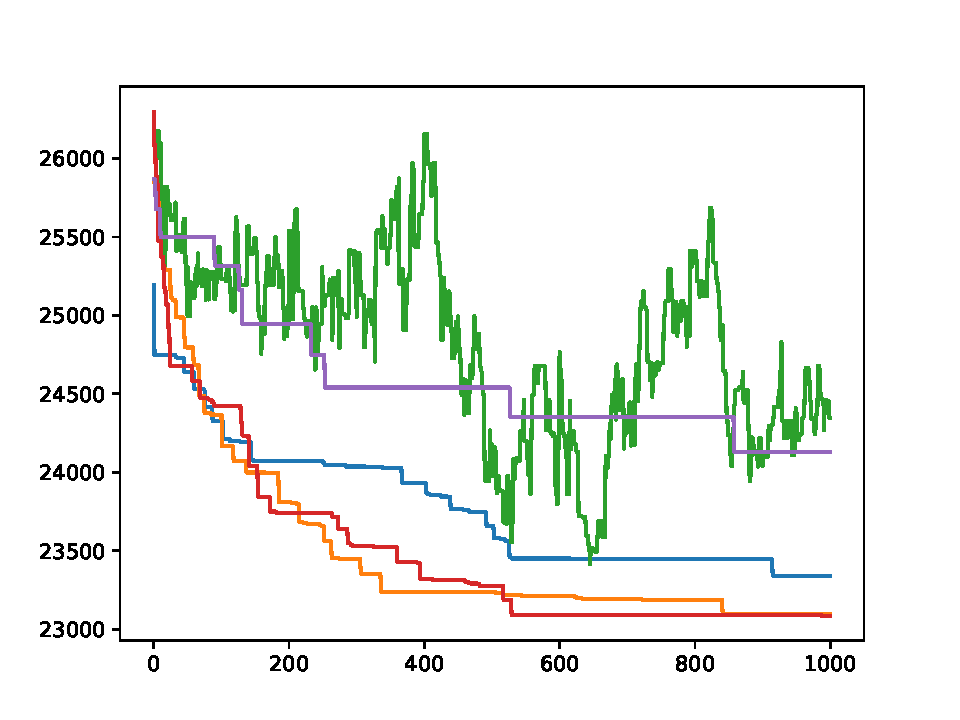
\includegraphics[scale=.6]{../Plots/new/5,2,multiple,eofb1000t-150.pdf}
\caption{Comparaison for $\lambda = 5$, $\mu = 2$ and multiple variation of
classic elitist selection (in blue), elitist selection on offsprings (in
orange), fitness proportional (in green), Boltzmann with constant $T = 1000$
(in red) and Threshold selection with constant parameter $T = -150$ (in
purple)}
\label{Multiplecompareselection}
\end{figure}

\subsection{Selections}

In figure~\ref{Elitistcomparevariation} and
figure~\ref{Offspringscomparevariation}, we observe that the mutation variation
and the mix of both variation and crossover yield interesting results.
Crossover doesn't look as good.
\\
In figure~\ref{Fitnesscomparevariation}, we can see that as predicted, my
fitness proportional selection stays quite uniform and non interesting.
\\
In figure~\ref{Boltzmanncomparevariation}, once again the crossover isn't
working so well. The two other variations are working well.
\\
In figure~\ref{Thresholdcomparevariation}, we can observe that the threshold
selection performs big steps, meaning that my $T$ variable could have been set
a little too big.
\\
In figure~\ref{Threshold-80comparevariation}, I reduced the $T$ variable. We
can observe smaller steps, thus converging faster to a better solution.

%ELITIST
\begin{figure}
\centering
%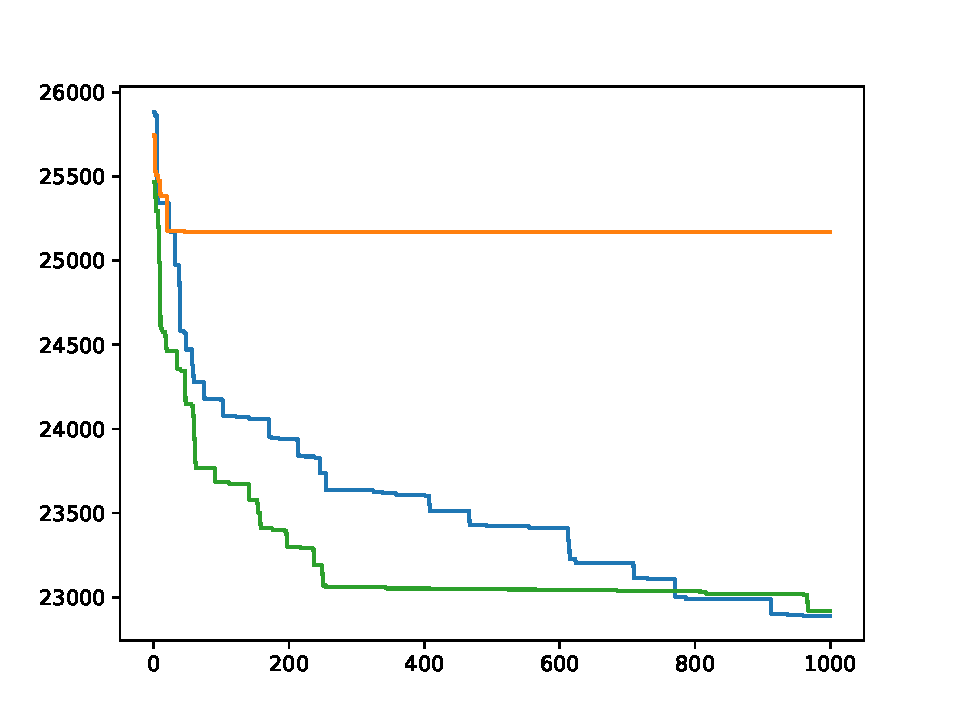
\includegraphics[scale=.6]{../Plots/5,2,elitist,mutcrossmult.pdf}
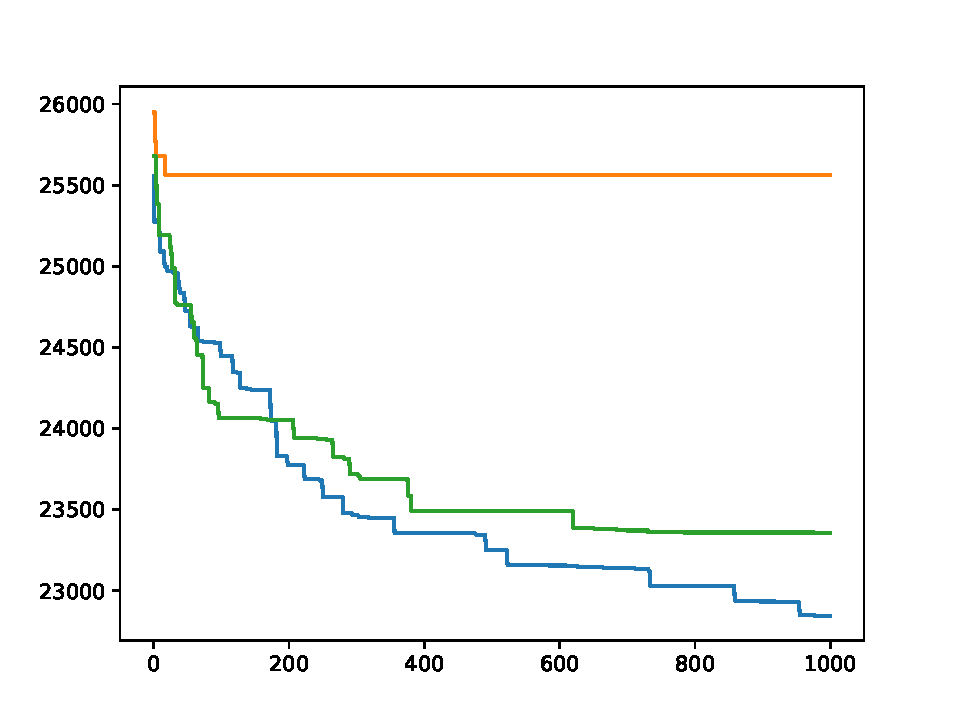
\includegraphics[scale=.6]{../Plots/new/5,2,mutcmul,elitist.pdf}
\caption{Comparaison for $\lambda = 5$, $\mu = 2$ and classic elitist selection
of mutation variation (in blue), crossover variation (in orange)  and another
variation consisting of a mix of both (in green).}
\label{Elitistcomparevariation}
\end{figure}

%OFFSPRINGS
\begin{figure}
\centering
%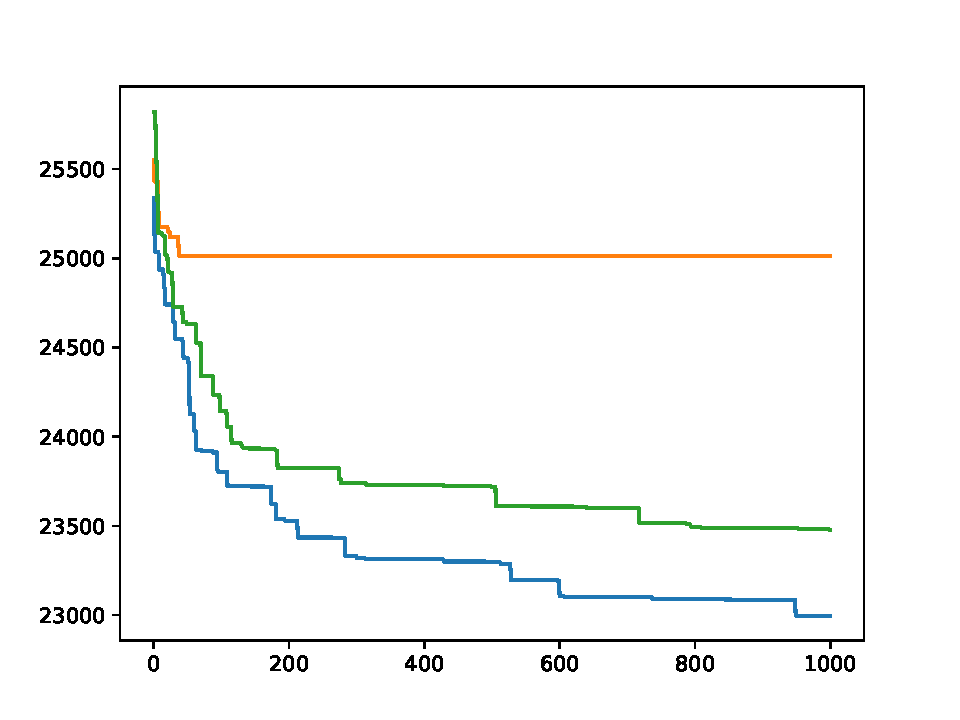
\includegraphics[scale=.6]{../Plots/5,2,offsprings,mutcrossmult.pdf}
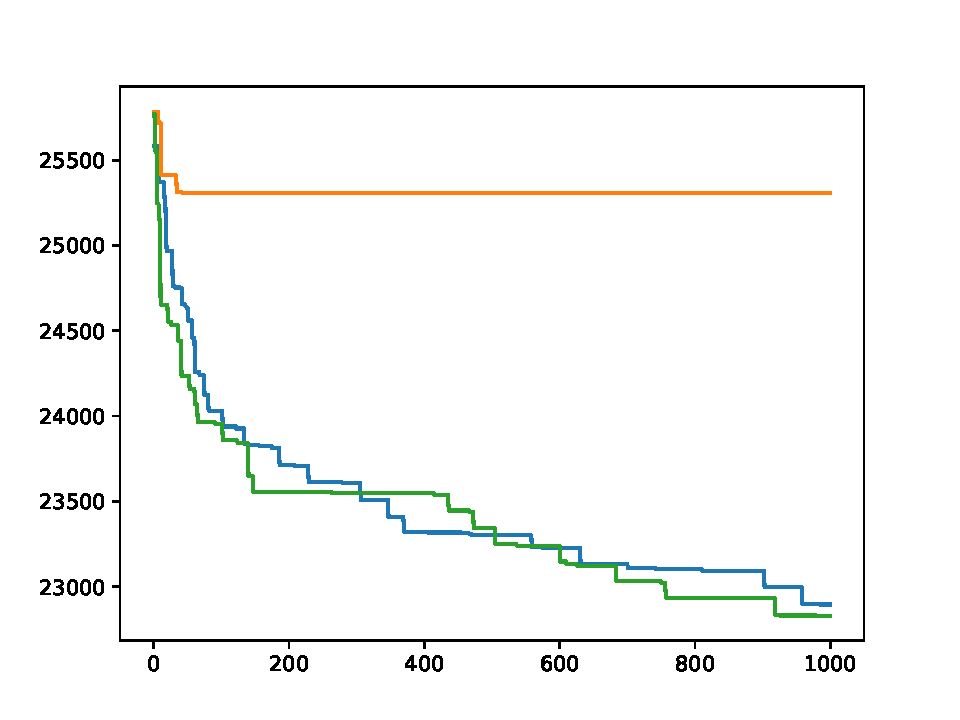
\includegraphics[scale=.6]{../Plots/new/5,2,mutcmul,offsprings.pdf}
\caption{Comparaison for $\lambda = 5$, $\mu = 2$ and offsprings elitist
selection of mutation variation (in blue), crossover variation (in orange)  and
another variation consisting of a mix of both (in green).}
\label{Offspringscomparevariation}
\end{figure}

%FITNESS
\begin{figure}
\centering
%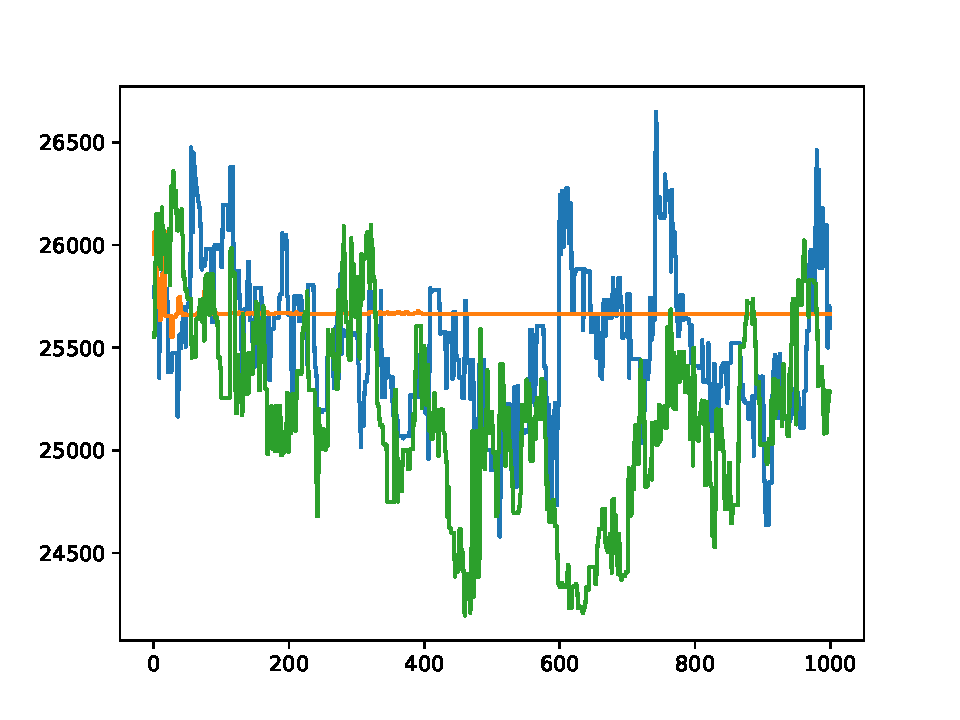
\includegraphics[scale=.6]{../Plots/5,2,fitness_prop,mutcrossmult.pdf}
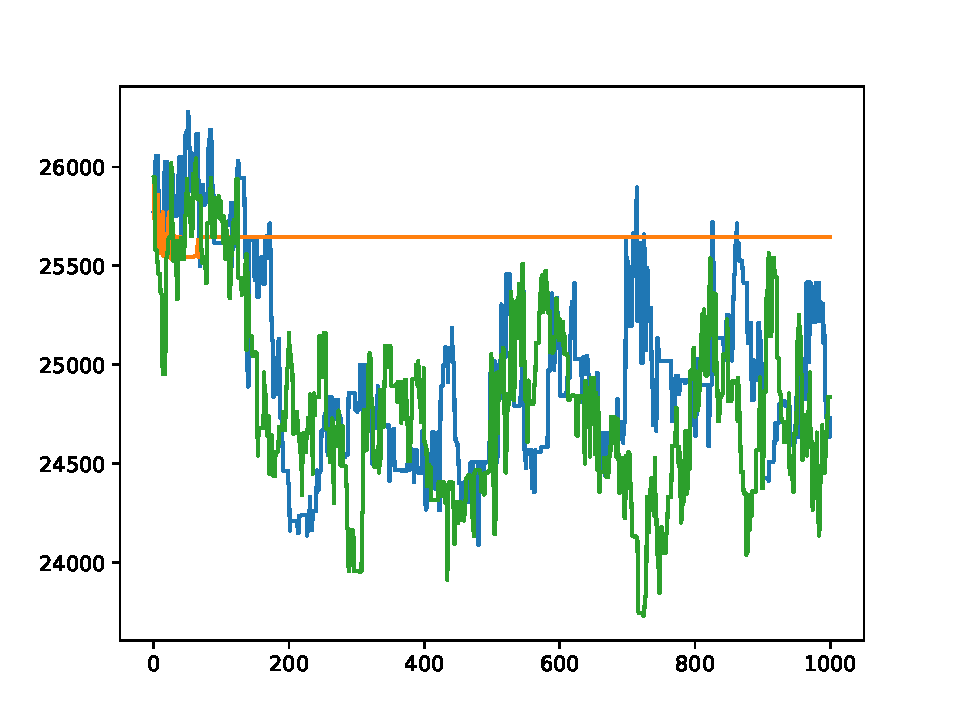
\includegraphics[scale=.6]{../Plots/new/5,2,mutcmul,fitness.pdf}
\caption{Comparaison for $\lambda = 5$, $\mu = 2$ and Fitness proportional
selection of mutation variation (in blue), crossover variation (in orange) and
another variation consisting of a mix of both (in green).}
\label{Fitnesscomparevariation}
\end{figure}

%BOLTZMANN
\begin{figure}
\centering
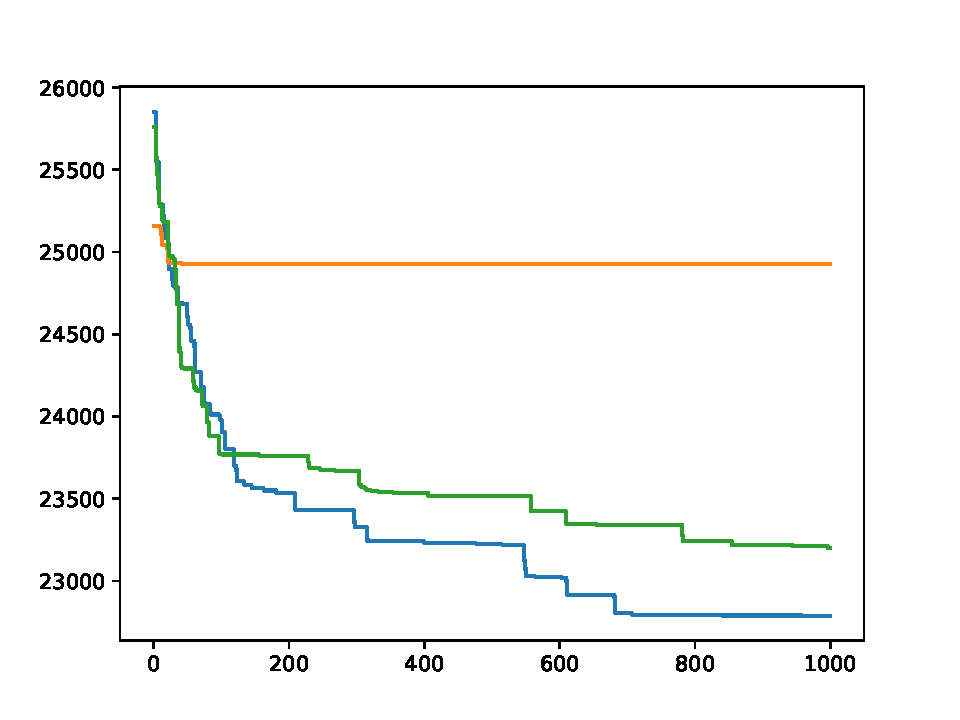
\includegraphics[scale=.6]{../Plots/new/5,2,mutcmul,Boltzmann1000.pdf}
\caption{Comparaison for $\lambda = 5$, $\mu = 2$ and Boltzmann selection with
constant parameter $T = 1000$ of mutation variation (in blue), crossover
variation (in orange) and another variation consisting of a mix of both (in
green).}
\label{Boltzmanncomparevariation}
\end{figure}

%THRESHOLD
\begin{figure}
\centering
%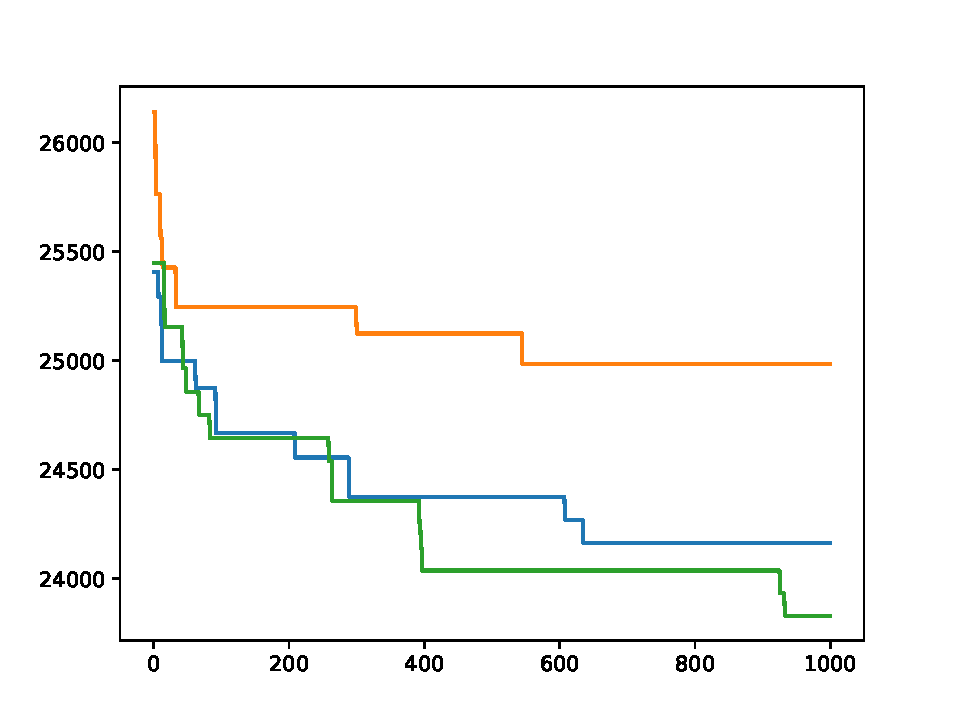
\includegraphics[scale=.6]{../Plots/5,2,Threshold-100,mutcrossmult.pdf}
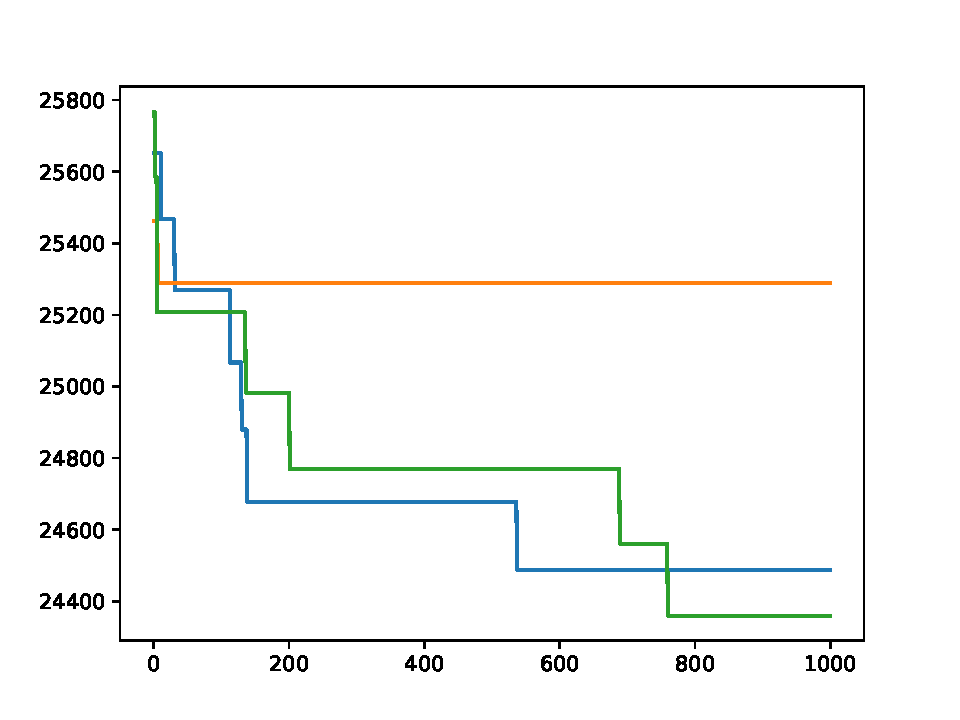
\includegraphics[scale=.6]{../Plots/new/5,2,mutcmul,threshold-150.pdf}
\caption{Comparaison for $\lambda = 5$, $\mu = 2$ and threshold selection with
constant parameter $T = -150$ of mutation variation (in blue), crossover
variation (in orange) and another variation consisting of a mix of both (in
green).}
\label{Thresholdcomparevariation}
\end{figure}

\begin{figure}
\centering
%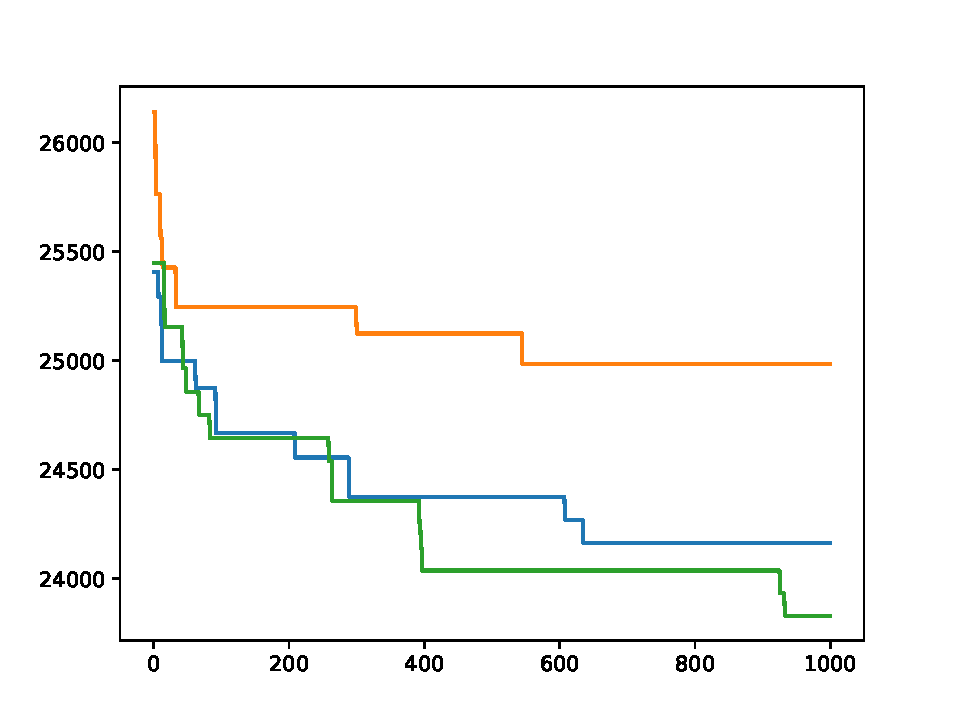
\includegraphics[scale=.6]{../Plots/5,2,Threshold-100,mutcrossmult.pdf}
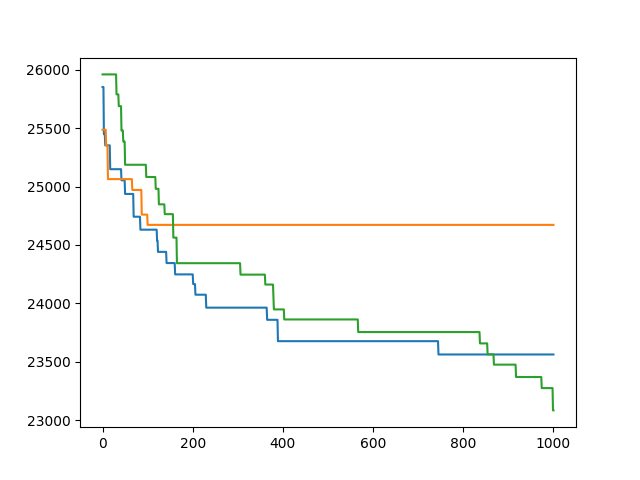
\includegraphics[scale=.6]{../Plots/new/5,2,mutcmul,Threshold-80.png}
\caption{Comparaison for $\lambda = 5$, $\mu = 2$ and threshold selection with
constant parameter $T = -80$ of mutation variation (in blue), crossover
variation (in orange) and another variation consisting of a mix of both (in
green).}
\label{Threshold-80comparevariation}
\end{figure}
\section{Conclusion}

For this problem, it looks like my fitness proportional and crossover
techniques aren't working very well. I am not sure why my crossover technique
isn't showing good results.

Techniques that seem to be working well are mutation variation and Boltzmann
selection.

Let's perform one last try with mutation variation and Boltzmann for $\lambda
= 11 $ and $\mu = 3$. See figure~\ref{MutationBoltzmann}

\begin{figure}
\centering
%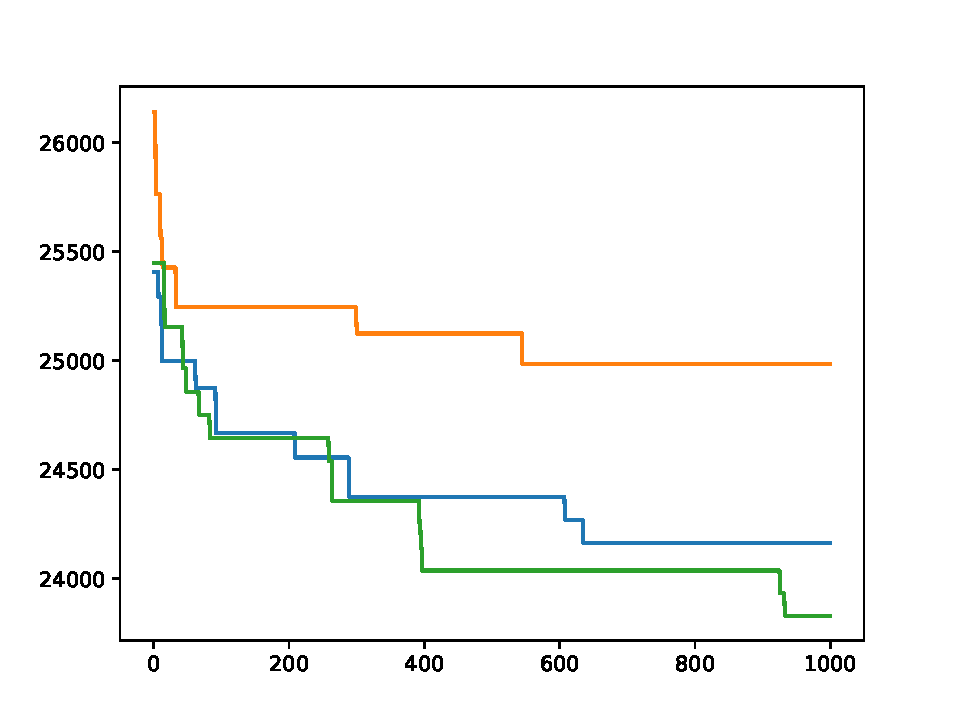
\includegraphics[scale=.6]{../Plots/5,2,Threshold-100,mutcrossmult.pdf}
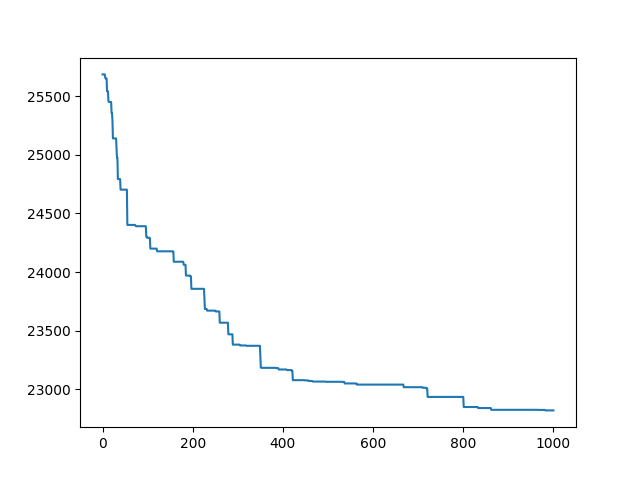
\includegraphics[scale=.6]{../Plots/new/11,3,mut,Boltzmann.png}
\caption{Comparaison for $\lambda = 11$, $\mu = 3$ and Boltzmann selection with
constant parameter $T = 1000$ and mutation variation (in blue)}
\label{MutationBoltzmann}
\end{figure}

\end{document}

